% PRL look and style (easy on the eyes)
\documentclass[aps,pre,twocolumn,nofootinbib,superscriptaddress,linenumbers]{revtex4-1}
% Two-column style (for submission/review/editing)
%\documentclass[aps,prl,preprint,nofootinbib,superscriptaddress,linenumbers]{revtex4-1}

\pdfoutput=1
\usepackage[pdftex]{graphicx}

\usepackage{alltt}

%\usepackage{palatino}

%\usepackage{palatino}
% Change to a sans serif font.
\usepackage{sourcesanspro}
\renewcommand*\familydefault{\sfdefault} %% Only if the base font of the document is to be sans serif
\usepackage[T1]{fontenc}
%\usepackage[font=sf,justification=justified]{caption}
\usepackage[font=sf]{floatrow}

% Rework captions to use sans serif font.
\makeatletter
\renewcommand\@make@capt@title[2]{%
 \@ifx@empty\float@link{\@firstofone}{\expandafter\href\expandafter{\float@link}}%
  {\sf\textbf{#1}}\sf\@caption@fignum@sep#2\quad
}%
\makeatother

\usepackage{listings} % For code examples
\usepackage[usenames,dvipsnames,svgnames,table]{xcolor}

\usepackage{amsmath}
\usepackage{amssymb}
%\usepackage[mathbf,mathcal]{euler}
%\usepackage{citesort}
\usepackage[caption=false]{subfig}
\usepackage{dcolumn}
\usepackage{boxedminipage}
\usepackage{verbatim}
\usepackage[colorlinks=true,citecolor=blue,linkcolor=blue]{hyperref}
\usepackage[group-separator={,}]{siunitx}

%Strikethrough
\usepackage{ulem}

% Justification
\captionsetup{singlelinecheck=off}

% Pretty-printing of shell commands
\newcommand{\shellcmd}[1]{\\\ \texttt{\scriptsize #1}}

% The figures are in a figures/ subdirectory.
\graphicspath{{../figures/}}

%% DOCUMENT %%%%%%%%%%%%%%%%%%%%%%%%%%%%%%%%%%%%%%%%%%%%%%%%%%%%%%%%%%%%%%%%%%%%
\begin{document}

%% TITLE %%%%%%%%%%%%%%%%%%%%%%%%%%%%%%%%%%%%%%%%%%%%%%%%%%%%%%%%%%%%%%%%%%%%
\title{Modeling experimental error in assays: Understanding discrepancies between assay results with different dispensing technologies}

\author{Sonya M. Hanson}
  \affiliation{Computational Biology Program, Sloan Kettering Institute, Memorial Sloan Kettering Cancer Center, New York, NY 10065, United States}
\author{Sean Ekins}
  \affiliation{Collaborations in Chemistry, Fuquay-Varina, NC 27526, United States}
\author{John D. Chodera}
 \thanks{Corresponding author}
 \email{john.chodera@choderalab.org}
  \affiliation{Computational Biology Program, Sloan Kettering Institute, Memorial Sloan Kettering Cancer Center, New York, NY 10065, United States}

\date{\today}

%%%%%%%%%%%%%%%%%%%%%%%%%%%%%%%%%%%%%%%%%%%%%%%%%%%%%%%%%%%%%%%%%%%%%%%%%%%%%%%%%%%%%%%%%%%%%%%%%%%%%%
% ABSTRACT/pacs
%%%%%%%%%%%%%%%%%%%%%%%%%%%%%%%%%%%%%%%%%%%%%%%%%%%%%%%%%%%%%%%%%%%%%%%%%%%%%%%%%%%%%%%%%%%%%%%%%%%%%%
\begin{abstract}

All experimental assay data is contaminated with error, but understanding the magnitude, type, and primary origin of this error is not often obvious.
Here, we describe a simple set of assay modeling techniques that allow sources of error and bias to be simulated and propagated into assay results.
We demonstrate how deceptively simple operations---such as the creation of a dilution series with a robotic liquid handler---can significantly amplify imprecision and even contribute substantially to bias.
To illustrate these techniques, we review an infamous example of how choice of dispensing technology can greatly impact assay measurements, and show how the primary contributions to discrepancies between assay results can be easily understood.
These simple modeling techniques---illustrated with an accompanying IPython notebook---can allow modelers making use of experimental data to understand the expected error and bias in the dataset, and even help experimentalists during the assay design stage to ensure that assays are capable of reaching their target accuracy and imprecision goals.

\end{abstract}

\maketitle

%%%%%%%%%%%%%%%%%%%%%%%%%%%%%%%%%%%%%%%%%%%%%%%%%%%%%%%%%%%%%%%%%%%%%%%%%%%%%%%%%%%%%%%%%%%%%%%%%%%%%%
% INTRODUCTION
%%%%%%%%%%%%%%%%%%%%%%%%%%%%%%%%%%%%%%%%%%%%%%%%%%%%%%%%%%%%%%%%%%%%%%%%%%%%%%%%%%%%%%%%%%%%%%%%%%%%%%
\section{Introduction}
\label{section:introduction}

Measuring the activity and potency of ligands---whether in biophysical or cell-based assays---is a critical step in optimizing small molecules for use as chemical probes or potential therapeutics, and indeed in probing biological processes in general.
All data are imperfect; use of this assay data for any purpose is invariably complicated by the fact that all assay data are contaminated with error, with contributions arising from numerous sources.

Often, the dominant contributions to assay error are simply not known---this is unsurprising, given the number and variety of potential contributing factors.
Even for what might be considered a straightforward assay involving fluorescent measurements of a ligand binding to a protein target, this might include (but is by no means limited to): compound impurities and degradation~\cite{kozikowski_effect_2003,kozikowski_effect_2003-1,cheng_studies_2003,waybright_overcoming_2009}, imprecise compound dispensing, unmonitored water absorption by DMSO stocks, the effect of DMSO on protein stability~\cite{tjernberg_dmso-related_2005}, intrinsic compound fluorescence~\cite{simeonov_fluorescence_2008,baell_new_2010}, compound insolubility~\cite{di_biological_2006} or aggregation~\cite{mcgovern_common_2002,mcgovern_kinase_2003,feng_high-throughput_2005,feng_synergy_2006,baell_new_2010}, variability in protein concentration or quality, pipetting errors, and inherent noise in any fluorescence measurement---not to mention stray lab coat fibers as fluorescent contaminants~\cite{busch_does_2015}. 
In an ideal world, a number of control experiments would be run to measure the magnitude of these effects, and data quality checks would either reject flawed data or ensure that all contributions to error have been carefully accounted for in producing an assessment of error and confidence for each assayed value.

%Often computational chemists are faced with comparing their models to experimental assay data for which there is no clear idea of the magnitude of the error. Sometimes no error is provided. Sometimes only a ballpark estimate is given. It would be useful to be able to get an estimate of how confident one should be in the data they are looking at. Other times, one might want to ensure ahead of time that an assay will produce useful data. For example if the error is larger than the dynamic range of the expected measurements, the assay will not be very useful.

Unfortunately, by the time the data reach the hands of a modeler (or other data consumer), the opportunity to perform these careful control experiments has passed, and yet somehow, one is expected to make good use of the data.
In the worst case, the communicated assay data may not contain any estimate of error whatsoever, making it fiendishly difficult to draw conclusions from the data---is the difference between multiple assay values for closely related compounds due to a true structure-activity relationship driving potency, or simply due to random error?
While aggregating many datasets can give a crude estimate of the general reliability of similar assays~\cite{kramer_experimental_2012,kalliokoski_comparability_2013}, knowledge of how a particular assay was conducted can inform the construction of an assay-specific model incorporating some of the dominant contributions to error in a manner that can be suprisingly informative.

%In many papers and reports errors or not provided or are inadequately explained. Our understanding of the reliability of experimental measurements of ligand binding affinity would be greatly increased if it was common practice to calculate expected experimental errors resulting from the major known sources.


In this paper, we review some common sources of error in experimental assays, and describe some simple modeling tools for simulating a model of an assay that incorporates these important (often dominant) sources of error. 
This approach, while simple, should nevertheless provide a powerful tool for modelers to understand how assay error depends on important parameters, such as providing a means to estimate the expected data error as a function of compound affinity.
Not only modelers may find benefit in this approach---these tools can be also used to help optimize assay formats before an experiment is performed, help troubleshoot problematic assays after the fact, or ensure that all major sources of error accounted for by checking that variations among controls match expectations.

We illustrate these concepts by considering a now-infamous example from the literature: a report by Ekins et al.~\cite{ekins_dispensing_2013} on how the choice of dispensing technology impacts the apparent biological activity of the same set of compounds under otherwise identical conditions.
The datasets employed in the analyses [CITE] used either a standard liquid handler with fixed (washable) tips or an acoustic droplet dispensing device to prepare the assay, resulting in highly divergent assay results (Figure~\ref{figure:overview}).
While the frustration for modelers was particularly great, since QSAR models derived from these otherwise identical assays produce surprisingly divergent predictions, numerous practitioners from all corners of drug discovery expressed their frustration in ensuing blog posts and commentaries~\cite{in-the-pipeline-comments}.
Hosts of potential reasons were speculated~\cite{in-the-pipeline-comments}, including [LIST HERE].

We make use this real-world example to illustrate some of the basic concepts behind modeling the most common sources of error in assays.
For simplicity, we ask whether the most basic contributions to assay error---imprecision and bias in material transfer operations and imprecision in measurement---might account for some component of this discrepancy between assay techniques.
We make use of very basic information---the assay protocol as described (with some additional inferences based on basic concepts such as compound solubility limits) and manufacturer specifications for imprecision and bias---to construct a model of each dispensing process to determine the overall inaccuracy and imprecision of the assay as a function of true compound affinity, and identify the steps that contribute the most to these assay data errors.
To better illustrate these techniques, we also provide an annotated IPython notebook that includes all of the computations described here in detail.
Readers are encouraged to download these notebooks and play with them to see how different assay configurations affect assay error.

\begin{figure*}[tb]
   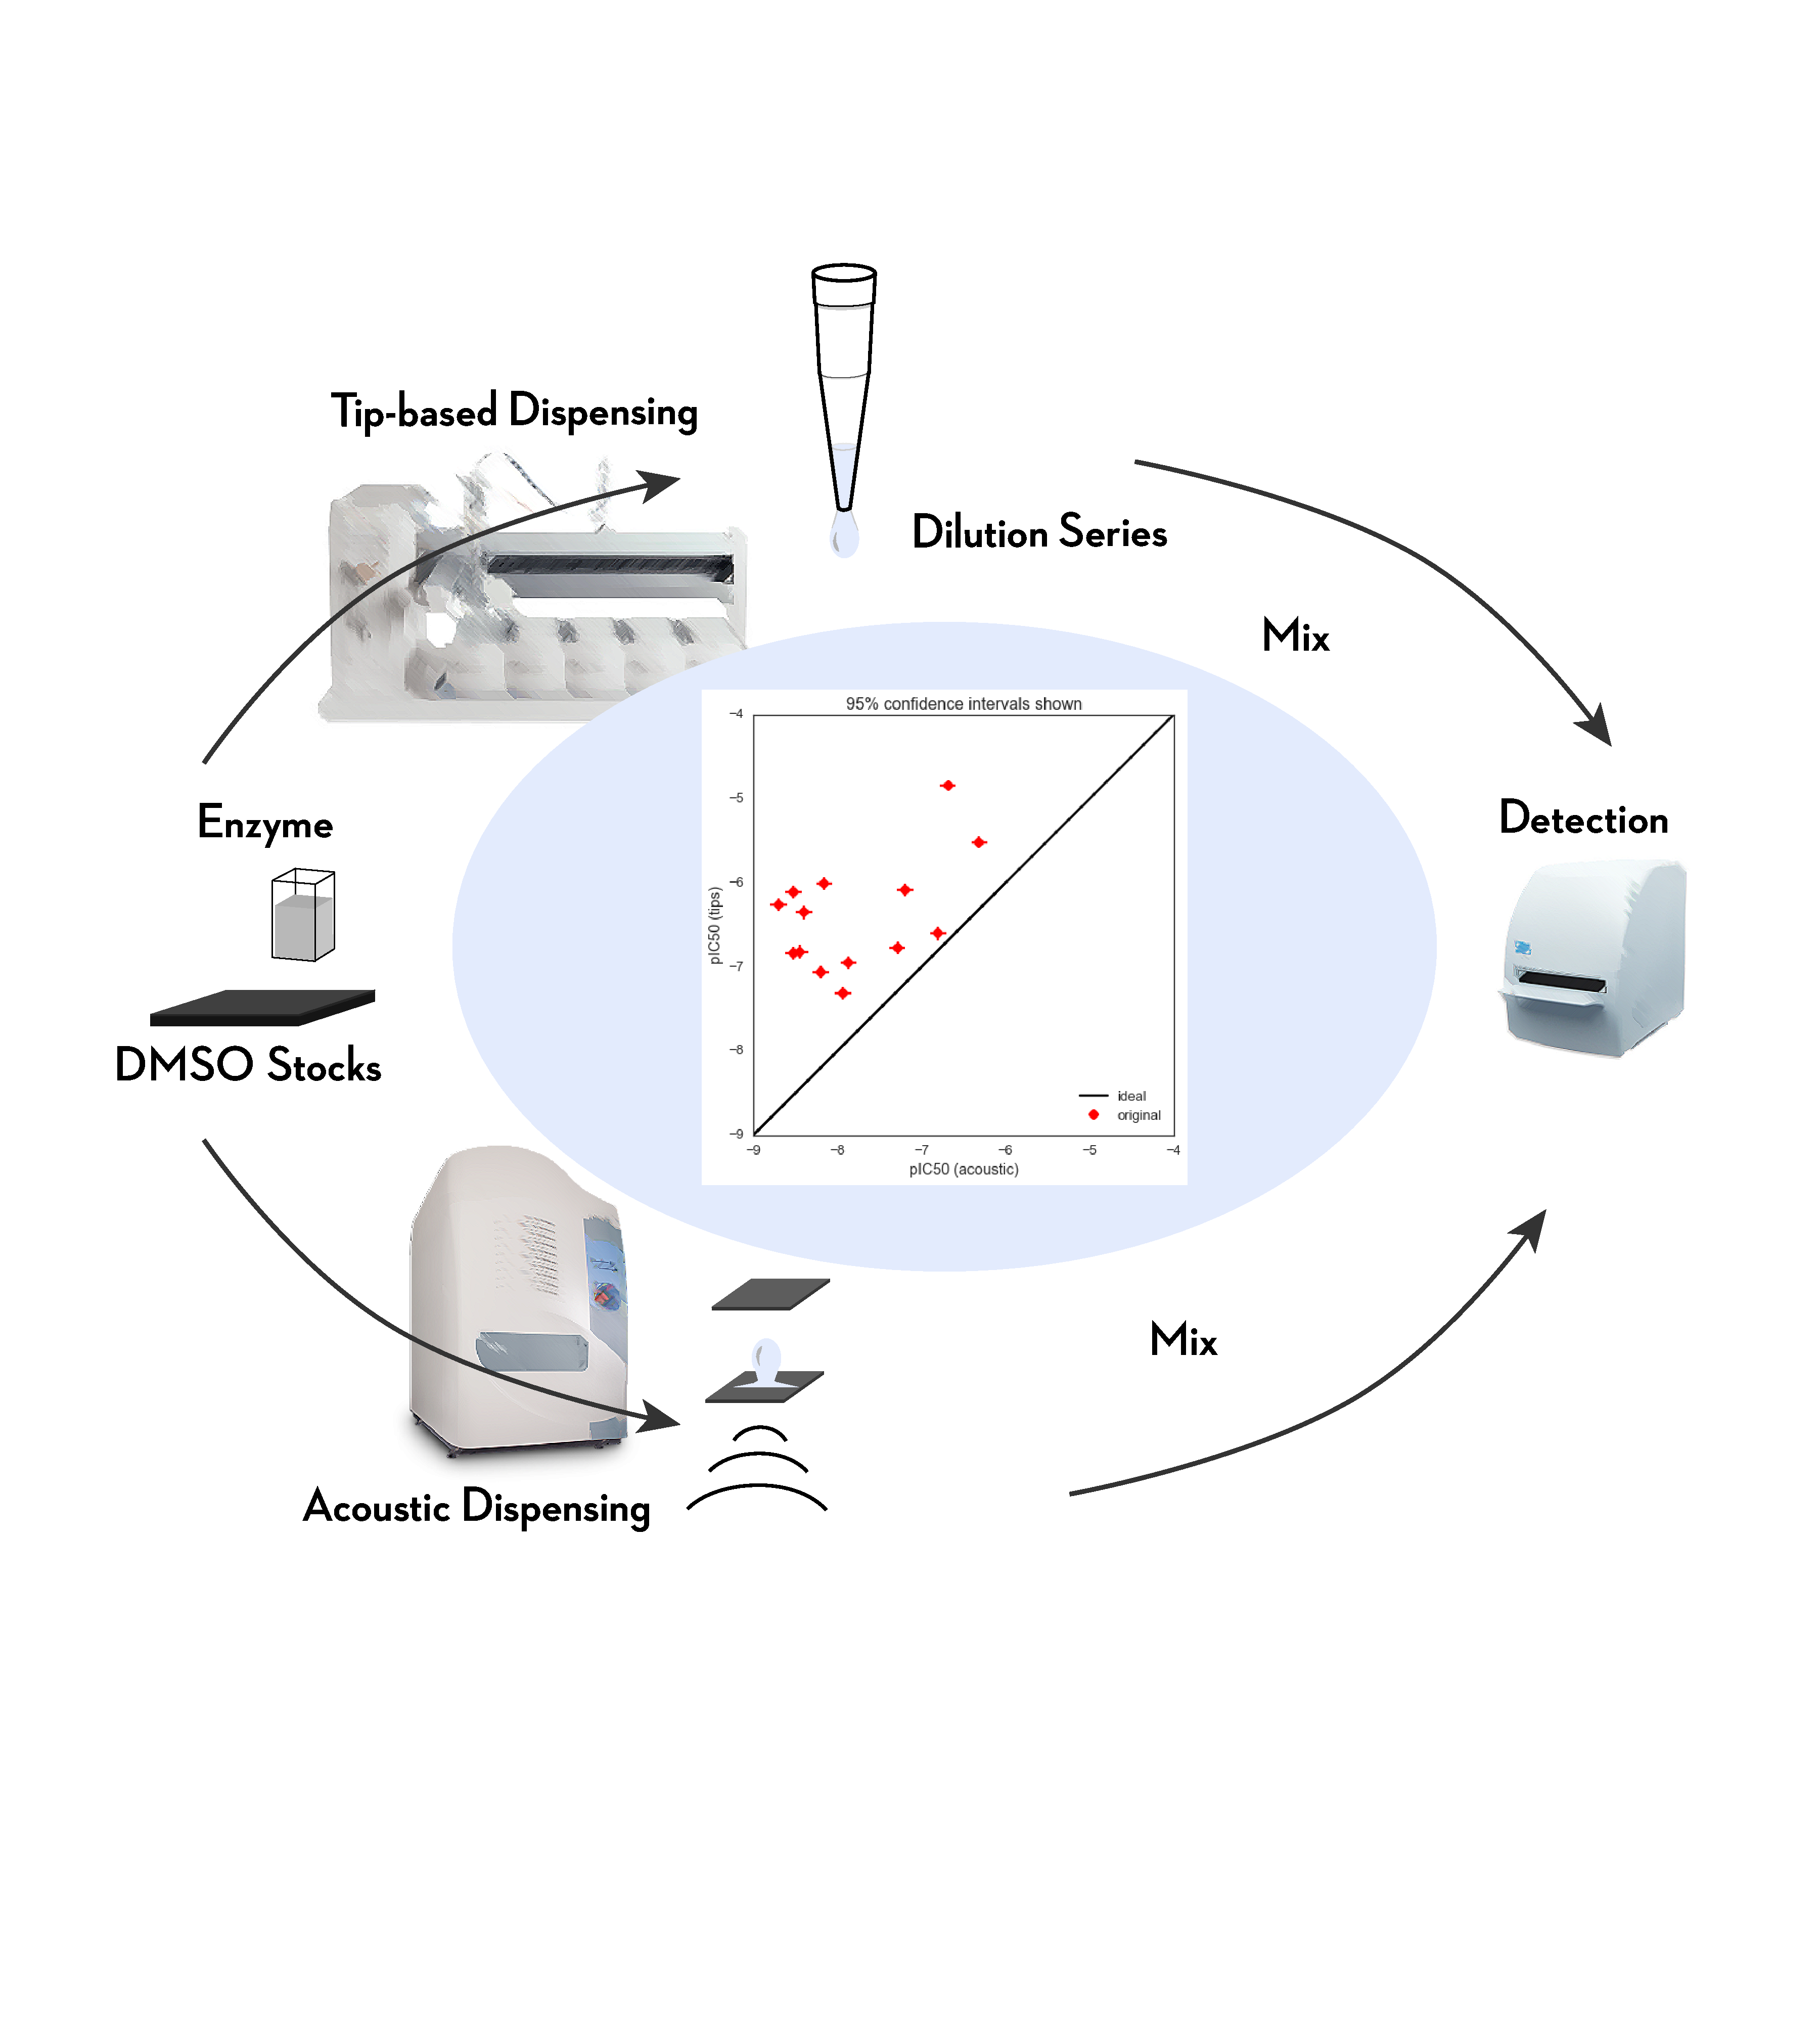
\includegraphics[trim={0 15cm 0 10cm},clip,width=0.75\textwidth]{../figures/Fig1-2.pdf}
  \caption{{\bf Diagrammatic representation of the various stages of the Ensembler pipeline and illustrative statistics for modeling all human tyrosine kinase catalytic domains.}
  On the left, the various stages of the {\bf Ensembler} pipeline are shown.
  On the right, the number of viable models surviving each stage of the pipeline is shown for modeling all 90 tyrosine kinases (\emph{All TKs}) and representative individual tyrosine kinases (\emph{SRC} and \emph{ABL}).
  Typical timings on a computer cluster (containing Intel Xeon E5-2665 2.4GHz hyperthreaded processors and NVIDIA GTX-680 or GTX-Titan GPUs) is reported to illustrate resource requirements per model for modeling the entire set of tyrosine kinases.
  Note that \emph{CPU-h} denotes the number of hours consumed by the equivalent of a single CPU hyperthread and \emph{GPU-h} on a single GPU---parallel execution via MPI reduces wall clock time nearly linearly.
  }
  \label{overview}
\end{figure*}


%%%%%%%%%%%%%%%%%%%%%%%%%%%%%%%%%%%%%%%%%%%%%%%%%%%%%%%%%%%%%%%%%%%%%%%%%%%%%%%%%%%%%%%%%%%%%%%%%%%%%
% Experimental error
%%%%%%%%%%%%%%%%%%%%%%%%%%%%%%%%%%%%%%%%%%%%%%%%%%%%%%%%%%%%%%%%%%%%%%%%%%%%%%%%%%%%%%%%%%%%%%%%%%%%%
\section{Experimental error}

Overall experimental error can be broken into two components: The \emph{imprecision} (or variance), which characterizes the random component of the error that causes different replicates of the same assay to give slightly different results, and the \emph{inaccuracy} (or bias), which is the deviation of the average over many replicates from the true value of the quantity being measured.

There are a variety of sources of experimental error... (figure out here what should be here, and what should be in intro).


\section*{Modeling experimental error}

Modeling experimental error is as simple as adding known values for imprecision and inaccuracy into a known assay. 

\subsection*{Simple liquid handling: Mixing solutions}

When an assay involves mixing two compounds together, as with most assays, you also have to consider mixing efficiency. For example if an assay involves mixing compound stock with a protein solution, usually a small volume into a much larger volume, uneven mixing can cause wide variation in the results. Several examples of this have been seen where, bla, bla, bla [ref,ref,ref]. Rules for propagation of error. Mention that the difficulties in mixing are not even considered in our simple model (we just assume good mixing).

\subsection*{Complex liquid handling: Dilution series}

Dilution series are often used to characterize the activity and potency of ligands. In dilution series, however, experimental errors are compounded, because the errors at an initial step of the dilution series will carry through to the next step. For example a 10\% error when transferring 50 uL from an initial stock to 50 uL of buffer to make a 1:2 dilution, will then end up being a blank \% total error once the 8th part of the dilution series is made. Explain bias and CV. CV's are amplified with each dilution

\subsubsection*{For a multichannel liquid-handler.}

To use more realistic numbers, for the Tecan Genesis the imprecision is stated as blank and the inaccuracy as blank, which means that if we're doing a blank blank, we will get blank (Figure~\ref{figure:acoustic-vs-tips}).  

\subsubsection*{For acoustic dispensing technology.}

For acoustic dispensing, however, this accumulated error in a dilution series is not a factor, since each step of the dilution is pipetted separately and directly, with good precision and accuracy down to very low volumes, in the case of the LabCyte Echo (Figure~\ref{figure:acoustic-vs-tips}). Despite the promises of the LabCyte Echo, we can see that it's CV and biases are mostly similar to that of the Tecan Genesis, even taking into account compounded error in the dilution series.

\subsubsection*{Fixed tips and the dilution effect.}

Another aspect of dispensing with multichannel liquid-handler, is the possibility of the dilution effect when using liquid-based fixed-tip pipetting, such as on the Tecan Genesis. This dilution effect was previously characterize in blank et al (BMS paper(S?)), and we can use these values to improve our model for the error in the multichannel liquid-handler. We can easily see that including this error, significantly shifts the bias we see for tip-based dispensing (Figure~\ref{figure:acoustic-vs-tips}).

%\begin{figure*}[tb]
%    \includegraphics[width=1.0\textwidth]{pipeline/pipeline2}
%
%  \caption{{\bf Diagrammatic representation of the various stages of the Ensembler pipeline and illustrative statistics for modeling all human tyrosine kinase catalytic domains.}
%  On the left, the various stages of the {\bf Ensembler} pipeline are shown.
%  On the right, the number of viable models surviving each stage of the pipeline is shown for modeling all 90 tyrosine kinases (\emph{All TKs}) and representative individual tyrosine kinases (\emph{SRC} and \emph{ABL}).
%  Typical timings on a computer cluster (containing Intel Xeon E5-2665 2.4GHz hyperthreaded processors and NVIDIA GTX-680 or GTX-Titan GPUs) is reported to illustrate resource requirements per model for modeling the entire set of tyrosine kinases.
%  Note that \emph{CPU-h} denotes the number of hours consumed by the equivalent of a single CPU hyperthread and \emph{GPU-h} on a single GPU---parallel execution via MPI reduces wall clock time nearly linearly.
%  }
%  \label{acoustic-vs-tips}
%\end{figure*}

\subsection*{Modeling plate reader measurement}

When measuring readouts of fluorescence assays, it is important to take intrinsic error in plate reader measurement into account. All observations have error. Luckily most plate readers already have these stats on hand in their manuals. For example the $\___$ used in this example has a fluorescence detection threshold of $\__$ and an error of $\__$.

\subsection*{Modeling an enzymatic reaction}

Creating a simple model of a competition assay can be done using standard formulas, here assuming we have data for Vmax. Similar models can be created for different assay readouts.

\subsection*{Simple imprecision insufficient to explain the Ekins discrepancy}

Plotting the inaccuracies and imprecisions and how the differ for tip-based dispensing vs. direct dispensing is extremely useful, and allows us to understand the errors in our assay results a bit better. It is easy to see that simple difference in these values, even when including the compounded error of the dilution series, does not give us much insight into the striking differences seen in Ekins et al between tip-based and direct dispensing.

However, if we incorporate the final component of error in tip-based dispensing, the dilution effect, we can see that correcting for this bias in plotting IC50 shifts tip-based values more toward direct-dispensing derived values (Figure~\ref{figure:IC50_bias}).

%\begin{figure*}[tb]
%    \includegraphics[width=1.0\textwidth]{pipeline/pipeline2}
%
%  \caption{{\bf Diagrammatic representation of the various stages of the Ensembler pipeline and illustrative statistics for modeling all human tyrosine kinase catalytic domains.}
%  On the left, the various stages of the {\bf Ensembler} pipeline are shown.
%  On the right, the number of viable models surviving each stage of the pipeline is shown for modeling all 90 tyrosine kinases (\emph{All TKs}) and representative individual tyrosine kinases (\emph{SRC} and \emph{ABL}).
%  Typical timings on a computer cluster (containing Intel Xeon E5-2665 2.4GHz hyperthreaded processors and NVIDIA GTX-680 or GTX-Titan GPUs) is reported to illustrate resource requirements per model for modeling the entire set of tyrosine kinases.
%  Note that \emph{CPU-h} denotes the number of hours consumed by the equivalent of a single CPU hyperthread and \emph{GPU-h} on a single GPU---parallel execution via MPI reduces wall clock time nearly linearly.
%  }
%  \label{IC50_bias}
%\end{figure*}

NOTES:
Add a table with inaccuracy, imprecision, dilution errors numbers?
Be sure to add second section to each of these paragraphs explain replicate result.

%%%%%%%%%%%%%%%%%%%%%%%%%%%%%%%%%%%%%%%%%%%%%%%%%%%%%%%%%%%%%%%%%%%%%%%%%%%%%%%%%%%%%%%%%%%%%%%%%%%%%
% DISCUSSION
%%%%%%%%%%%%%%%%%%%%%%%%%%%%%%%%%%%%%%%%%%%%%%%%%%%%%%%%%%%%%%%%%%%%%%%%%%%%%%%%%%%%%%%%%%%%%%%%%%%%%
\section{DISCUSSION}

OUTLINE FROM GOOGLE DOC (TO BE MADE INTO PROSE IN THE FUTURE):
Why model assays?
during assay design: 
we can answer “will the assay meet my goals/needs?” before investing time or money
can identify unknowns that will affect assay utility, and measure them if needed
can better identify pilot experiments that will allow assay tuning (eg measure known compounds near expected assay limits)
during assay optimization: plug in measured uncertainties, optimize assay format
assay validation: do we understand all of the primary sources of error?
assay QC: are we reproducibly meeting our target behavior with our controls?
after an assay has been performed: how can I estimate the magnitude of error? 
useful for modellers / data consumers

Take-away messages:
it’s hard to make a good dilution series!
a large liquid handling CV can still result in a smaller overall assay CV
dilution effects can be important in liquid handling with fixed tips; can lead to large biases
direct dispensing techniques (Echo and D300) can be useful in reducing bias and error

Helpful resources:
pointers to our IPython notebooks
other useful resources for modeling assays


%%%%%%%%%%%%%%%%%%%%%%%%%%%%%%%%%%%%%%%%%%%%%%%%%%%%%%%%%%%%%%%%%%%%%%%%%%%%%%%%%%%%%%%%%%%%%%%%%%%%%
% ACKNOWLEDGMENTS
%%%%%%%%%%%%%%%%%%%%%%%%%%%%%%%%%%%%%%%%%%%%%%%%%%%%%%%%%%%%%%%%%%%%%%%%%%%%%%%%%%%%%%%%%%%%%%%%%%%%%
\section{Acknowledgments}
\label{section:acknowledgments}

Thanks to everybody!

%%%%%%%%%%%%%%%%%%%%%%%%%%%%%%%%%%%%%%%%%%%%%%%%%%%%%%%%%%%%%%%%%%%%%%%%%%%%%%%%%%%%%%%%%%%%%%%%%%%%%%
% BIBLIOGRAPHY
%%%%%%%%%%%%%%%%%%%%%%%%%%%%%%%%%%%%%%%%%%%%%%%%%%%%%%%%%%%%%%%%%%%%%%%%%%%%%%%%%%%%%%%%%%%%%%%%%%%%%%

\bibliographystyle{prsty} 
\bibliography{dispensing-errors.bib}


\end{document}
